\documentclass[12pt,a4paper,titlepage]{book}
% set line spacing to 1.5 and font to Times
\renewcommand{\baselinestretch}{1.5}
\usepackage{times}

\usepackage[
backend=biber,
style=ieee,
citestyle=ieee
]{biblatex}
\addbibresource{interim_references.bib}


\usepackage[pagestyles]{titlesec}
\titleformat{\chapter}{\normalfont\huge}{\thechapter.}{20pt}{\huge}
\titlespacing*{\chapter}{0pt}{-50pt}{40pt}

\newpagestyle{no-chapter-headers}{
  \sethead[\thepage][][\chaptertitle]{\thesection~\sectiontitle}{}{\thepage}
}
\pagestyle{no-chapter-headers}

\usepackage{graphicx}

\usepackage{pdfpages}

\begin{document}

\title{
  
\includegraphics[width=0.3\linewidth]{ul-logo.jpg}
  \hspace{1cm}
  
\includegraphics[width=0.6\linewidth]{ECE_Logo.png}
  %\centering
\includegraphics[width=14cm]{ECE_Logo.png}\\ [2ex]
  Machine Learning Using Python Frameworks\\ [2ex] 
  {\Large Interim Final Year Project Report}
}
\author{Lorcan Williamson\\Supervisor: Dr. K. Murphy}
%\date{October 27, 1995}
\maketitle

\tableofcontents

\chapter{Introduction and Project Description}
\section{Introduction}
	Machine learning has advanced hugely through the use of deep learning in recent years. This project aims to explore the landscape through Python machine learning frameworks such as Scikit-Learn, Tensorflow and Keras. This will be done by looking at examples of common machine learning problems and the steps taken to develop solutions using these frameworks.
\section{Project Outline}
	This project will examine how code is developed to solve problems in the two main use cases of machine learning; classification, and regression. The problems will be chosen to examine the most model architectures and development practices in as few problems as possible. To do this three problems have been chosen, two classification and one regression. \\
	The classification problems involve one image recognition problem\footnote{Detecting Pneumonia in chest X-rays} and one feature based problem\footnote{Determining student performance based on a number of factors}. Two classification problems were chosen to offer a use case for convolutional neural network (CNNs), which are used almost exclusively for machine vision problems. Another classification was also chosen so that other architectures could be examined, as it is uncommon to use CNNs on anything but image based problems. \\ \\
	The regression problem\footnote{Predicting Bitcoin prices based on historic data} was chosen to look at time-series problems, which are very often regression problems. This allows a look at architectures such as recurrent neural networks (RNNs) and long-short term memory (LSTM) networks, a special type of RNN. \\
	The datasets were chosen to try represent realistic problems machine learning would be used to solve instead of using one of the more common benchmarking datasets such as CIFAR-10\cite{cifar-10} or Iris, to create a more realistic example of the code development process, especially data preparation, which is often already done for common benchmarking datasets.


\chapter{Literature Survey}
\section{Problem Categories}
	This project focuses on code development for machine learning problems using python. Only supervised learning problems are being examined in this, due to supervised learning being faster and of comparable, if not better, accuracy for many non-linear classification problems as discussed in Bradley C Love's paper comparing supervised and unsupervised learning for classification problems\cite{supervised-vs-unsupervised}. Stephen Marsland's \textit{Machine Learning an Algorithmic Perspective (2\textsuperscript{nd} Edition)}\cite{ml-algorithmic-perspective} provided a good basis for many of the learning algorithms this project plans to look at. In it he categorises machine learning problems into two main categories; classification, and regression. It is for this reason that these are the two problem types discussed.
\section{Classification Problems}
	Classification problems involve the class of a presented input from a discrete number of predefined classes (labels), such as determining whether an image is of a dog or a cat, or determining the species of a plant given measurements taken from it. S.B Kotsianstis\cite{classification-techniques} discusses many of the common machine learning algorithms for use on classification problems, such as decision trees/random forests, support vector machines (SVMs), and artificial neural networks (ANNs), as well as many others.
\subsection{Machine Vision}
	Machine Vision covers a large number of problems, such as image-recognition, classification, object-detection, etc. This is an inherently classification type problem, rather than regression, and is one of the most common uses of machine learning in machine vision. In their 2012 paper \textit{ImageNet Classification with Deep Convolutional Neural Networks}\cite{image-net}, Alex Krizhevsky, Ilya Sutskever, and Geoffrey E Hinton showed that CNNs could achieve excellent results on image recognition tasks when compared to other machine learning or deep learning algorithms. This is what led to the choice to have two classification problems, an image-recognition problem and one other. Martin Thoma's master's thesis \textit{Analysis and Optimization of Convolutional Neural Network Architectures}\cite{cnn-analysis} offers a great deal of insight into the theory and implementation of convolutional neural networks.
\section{Regression Problems}
	Regression problems are problems of predicting values rather than classes, such as stock prices. Some regression problems can be converted to classification problems by quantising the output values into classes. \textit{An empirical comparison of machine learning models for time series forecasting (2010)}\cite{regression-techniques} compares a large number of models for forecasting values based on historic time-series data. This should be very useful for the regression problem examined in this project.

\chapter{Theory}
	While it will not be the main focus of this project, the theory of machine learning will still be important, and may be referenced at times. Here we shall look at some of the underlying theory that is used in the machine and deep learning algorithms that may be used or examined for use in solving the problems discussed in this project
\section{Overview of Machine Learning}
	Machine learning is a field in computer science concerned with developing algorithms that can allow a machine to solve problems by supplying data and teaching them to produce the desired output. There are three main teaching techniques; supervised, unsupervised, and reinforcement.\cite{ml-algorithmic-perspective} Supervised learning involves showing the machine a number of collections of features, presentations, and comparing the output observed to the desired output, or label. The machine can then update its parameters by following some algorithm to approach the desired output. Unsupervised learning is similar, however now no labels are provided, and the machine simply groups the presentations together based on their features, this means learning generally takes longer than supervised learning\cite{supervised-vs-unsupervised}, but not needing a labelled dataset can be advantageous, as it can often take a lot of time to manually label data. Semi-supervised learning has been explored in recent years, which uses partially labelled data, and seems to offer a good trade off between supervised and unsupervised learning\cite{semi-supervised}.\\
	Reinforcement learning is useful in machine learning tasks that require the machine to make decisions to reach a goal, for example in playing a game. The machine is asked to make a decision, and then rewarded if this decision brings it closer to that goal.
\section{Artificial Neural Networks}
	Artificial neural networks are machines made up of many artificial neurons. The basic model for an artificial neuron was described by McCulloch and Pitts in 1943\cite{mcculloch-pitts-neuron} (Figure 3.1). The McCulloch-Pitts neuron works by taking the weighted sum of the inputs, and putting this through some activation function to decide whether the neuron fires or not. A number of functions can be used for the activation, though sigmoid is one of the most common.
\begin{figure}[h!]
  \centering
  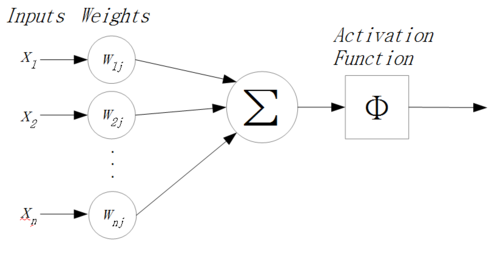
\includegraphics[width=0.7\linewidth]{mcculloch-pitts.png}
  \caption{The McCulloch-Pitts neuron}
  \label{fig:m-p-neuron}
\end{figure}\\
	This is the basic architecture used by a number of artificial neurons which use different algorithms to update the weights to learn to solve problems, such as the perceptron or adaline algorithms. A single neuron is capable of solving a linearly separable problem\cite{ml-algorithmic-perspective}. This isn't useful for most real world problems, but by stacking layers of neurons the problem can be reduced until the final layer needs to only solve a linearly separable problem. This is known as a multi-layer perceptron (MLP) if only dense perceptron layers are used, or an artificial neural network (ANN) in general\cite{intro-to-nn}. Deep neural networks are generally classified as any ANN with more than two dense hidden layers (weight layers between the inputs and the output neurons).\\
	There are again many algorithms used to train ANNs, most of which are based on the idea of gradient descent, which minimises the error by adjusting the weights to move towards a local minimum in the weight space\cite{back-prop}. More advanced methods may include some form of momentum term to avoid getting stuck on saddle points or shallow local minima.
\subsection{Convolutional Neural Networks}
	Convolutional neural networks are a type of MLP that are very good at image recognition, and in this description the inputs will be discussed as images, though the theory applies to any input type. They are made up of convolutional layers, that work by using matrices of weights, called \textit{kernels}. These allow the model to detect translational-invariant features, such as those in images, where the position of a feature is not important. By convolving the kernels with the image, features will be detected regardless of location. The kernels are in generally either 2 or 3 dimensional, depending on if the image is grey-scale or RGB, and typically either $3\times3$ or $5\times5$ ($\times3$ if the input is RGB)\cite{cnn-analysis}.\\
	Convolutional layers are often followed by \textit{pooling layers}, which are designed to reduce the size of the input, making it more feature dense. Pooling layers reduce the size of the image by taking the activation levels of the neurons in a (typically square) area, or \textit{pool}, and reduce these values to a single value. The two most common ways of reducing the activation weights is either through max-pooling, taking the maximum value in the pool, or average-pooling, taking the average of the weights\cite{cnn-analysis}. Pools are typically of size $2\times2$, and usually are not overlapping, though in general they can.
\section{Support Vector Machines}
	Support vector machines (SVMs), or support vector networks, were described by Corinna Cortes and Vladimir Vapnik in their 1995 paper \textit{Support-Vector Networks}\cite{support-vector-machines}. Its basic operation of a support vector machine was outlined as 
\begin{quote}
 	"[A support vector network] conceptually implements the following idea: input vectors are non-linearly mapped to a very high-dimension feature space. In this feature space a linear decision surface is constructed. Special properties of the decision surface ensures high generalization ability of the learning  machine."
\end{quote}
	This avoids one of the main problems of perceptrons, and other artificial neuron; the fact they can only solve linearly separable problems, by mapping the inputs to a higher dimensional space where they are linearly separable.\\
	SVMs allow for binary classification, though a multi-class SVM can be made from the combination of multiple binary SVMs, or using multi-class kernel-based vector machines\cite{multiclass-svm}. SVMs offer many advantages over other neural network training algorithms, such as gradient-descent. Chief of which is the training time, which is not based on the degree of the decision-surface polynomial, but only the number of support vectors. This gives a linear relationship for computational complexity versus the number of support vectors, compared to exponential for neural networks versus the number of layers.
\section{Decision Trees and Random Forests}
	Binary trees are a very common and well studied data-structure in computer science. Searching through a balanced binary tree is very efficient, $O(\log N)$, where $N$ is the number of nodes. Decision trees are binary trees constructed to classify data based on feature provided. This makes them very fast for querying once they have been constructed. There are a number of algorithms for constructing decision trees, such as ID3\cite{ID3} or CART\cite{CART}. These are usually greedy algorithms that focus on trying to separate the features to split the classes the most evenly. To do this they use some measure of informational entropy, which measures how much the data can be split by a single feature, which is a maximum when it splits the data is split in half\cite{info-entropy}.\\
	A random forest is a collection of decision trees, each trained on slightly different data. By training each decision tree on slightly different data, the overall forest becomes less sensitive to noise in the data. The output of the forest is then taken as the majority vote in the case of classification, or the mean response of each tree for regression. This can allow a number of low accuracy trees ($<70\%$), to achieve much higher accuracies ($>90\%$).

\chapter{Outline Design}
	This project will look at three different problems, two classification and one regression, and how one may go about solving them using Python machine learning frameworks. This will cover code development from examining and preparing the training data, through selecting and optimising learning algorithms to testing the chosen solution. So far the datasets for the problem have been selected, and examination of them has begun. The frameworks used for this project will be Scikit-Learn\footnote{https://scikit-learn.org/stable/index.html} and Keras\footnote{https://www.tensorflow.org/guide/keras}, a high-level API that can be built on top of, and is available in, Tensorflow.
\section{Classification Problem 1: Student Performance}
	The first problem examined is a classification problem predicting students performance in final year\cite{student-performance-dataset}. This dataset has quite high dimensionality\footnote{The dataset contains 31 features}, so will probably benefit from some dimensionality reduction technique such as principal PCA\footnote{Principal Component Analysis} or some similar technique\cite{dimensional-reductions}. It should be noted that one of the features of the dataset, feature 31, the first/second period grade might be ignored, due to it trivialising the problem given how strongly it correlates to the final grade. It may be examine however, as it will allow for very easy visualisation of the data and the way in which various classification algorithms separate it.
\section{Classification Problem 2: Detecting Pneumonia}
	The second classification problem involves detecting pneumonia in patients from images of chest x-rays\cite{pneumonia-dataset}. The images are binary classified, into \textit{Normal} and \textit{Pneumonia}. The Pneumonia images include cases of both viral and bacterial, but no distinction is made. There are 5216 images in the training data, 1341 examples of a normal x-ray, and 3875 examples of an x-ray with pneumonia. This means some class balancing technique such as those discussed in Mateusz Buda1's, Atsuto Maki's, and Maciej A. Mazurowski's 2018 paper on class imbalance problems in CNNs\cite{balancing-classes} may be required.
\section{Regression Problem: Bitcoin Prices}
	The last problem examined is a regression problem, predicting future trading prices of Bitcoin based on historical data\cite{bitcoin-dataset}\footnote{Available under Creative Commons license (https://creativecommons.org/licenses/by-sa/4.0/)}. The data included spans from January 2012 to August 2019, in one minute intervals, though some gaps exist in the data. There are also missing values for some entries. This may not be an issue, but if it is then some of the techniques discussed in \textit{A Review of Missing Values Handling Methods on Time-Series Data}\cite{missing-data} may be useful.

\chapter{Action plan}
	Planning for this project has been done using a Gantt chart, starting on 21/10/19 and ending 29/03/2020 (See next page). A description of the tasks, and approximately how much time is given to them, can be seen below. The student performance problem has been given extra as it coincides with end of semester exams.
\begin{enumerate}
\item \textbf{Explore Data}: This task is to examine the data for the problem, prepare code to allow it to be used with the Python frameworks, and perform any preprocessing required; such as normalisation, feature reduction, or class-balancing. Five days have been allocated for this task.
\item \textbf{Research Models}: During this time research will be done into how models were developed for similar problems, to narrow down the types of model that could be used in the development stage. Seven Days have been allocated for this.
\item \textbf{Develop \& Test Models}: During this time a number of models will be developed and tested using validation data as a metric for deciding which model to use. Fourteen days have been allocated for development and testing.
\item \textbf{Test \& Evaluate Final Model}: The final task for each example problem will be to test the final model chosen on the testing data, and evaluate its performance. Two days have been allocated for this.
\item \textbf{Write up of Final Report}: This task will be ongoing throughout the entire project. On the Gantt chart milestones have been set to have the write up for each example problem completed approximately one week after the completion of that problem.
\end{enumerate}
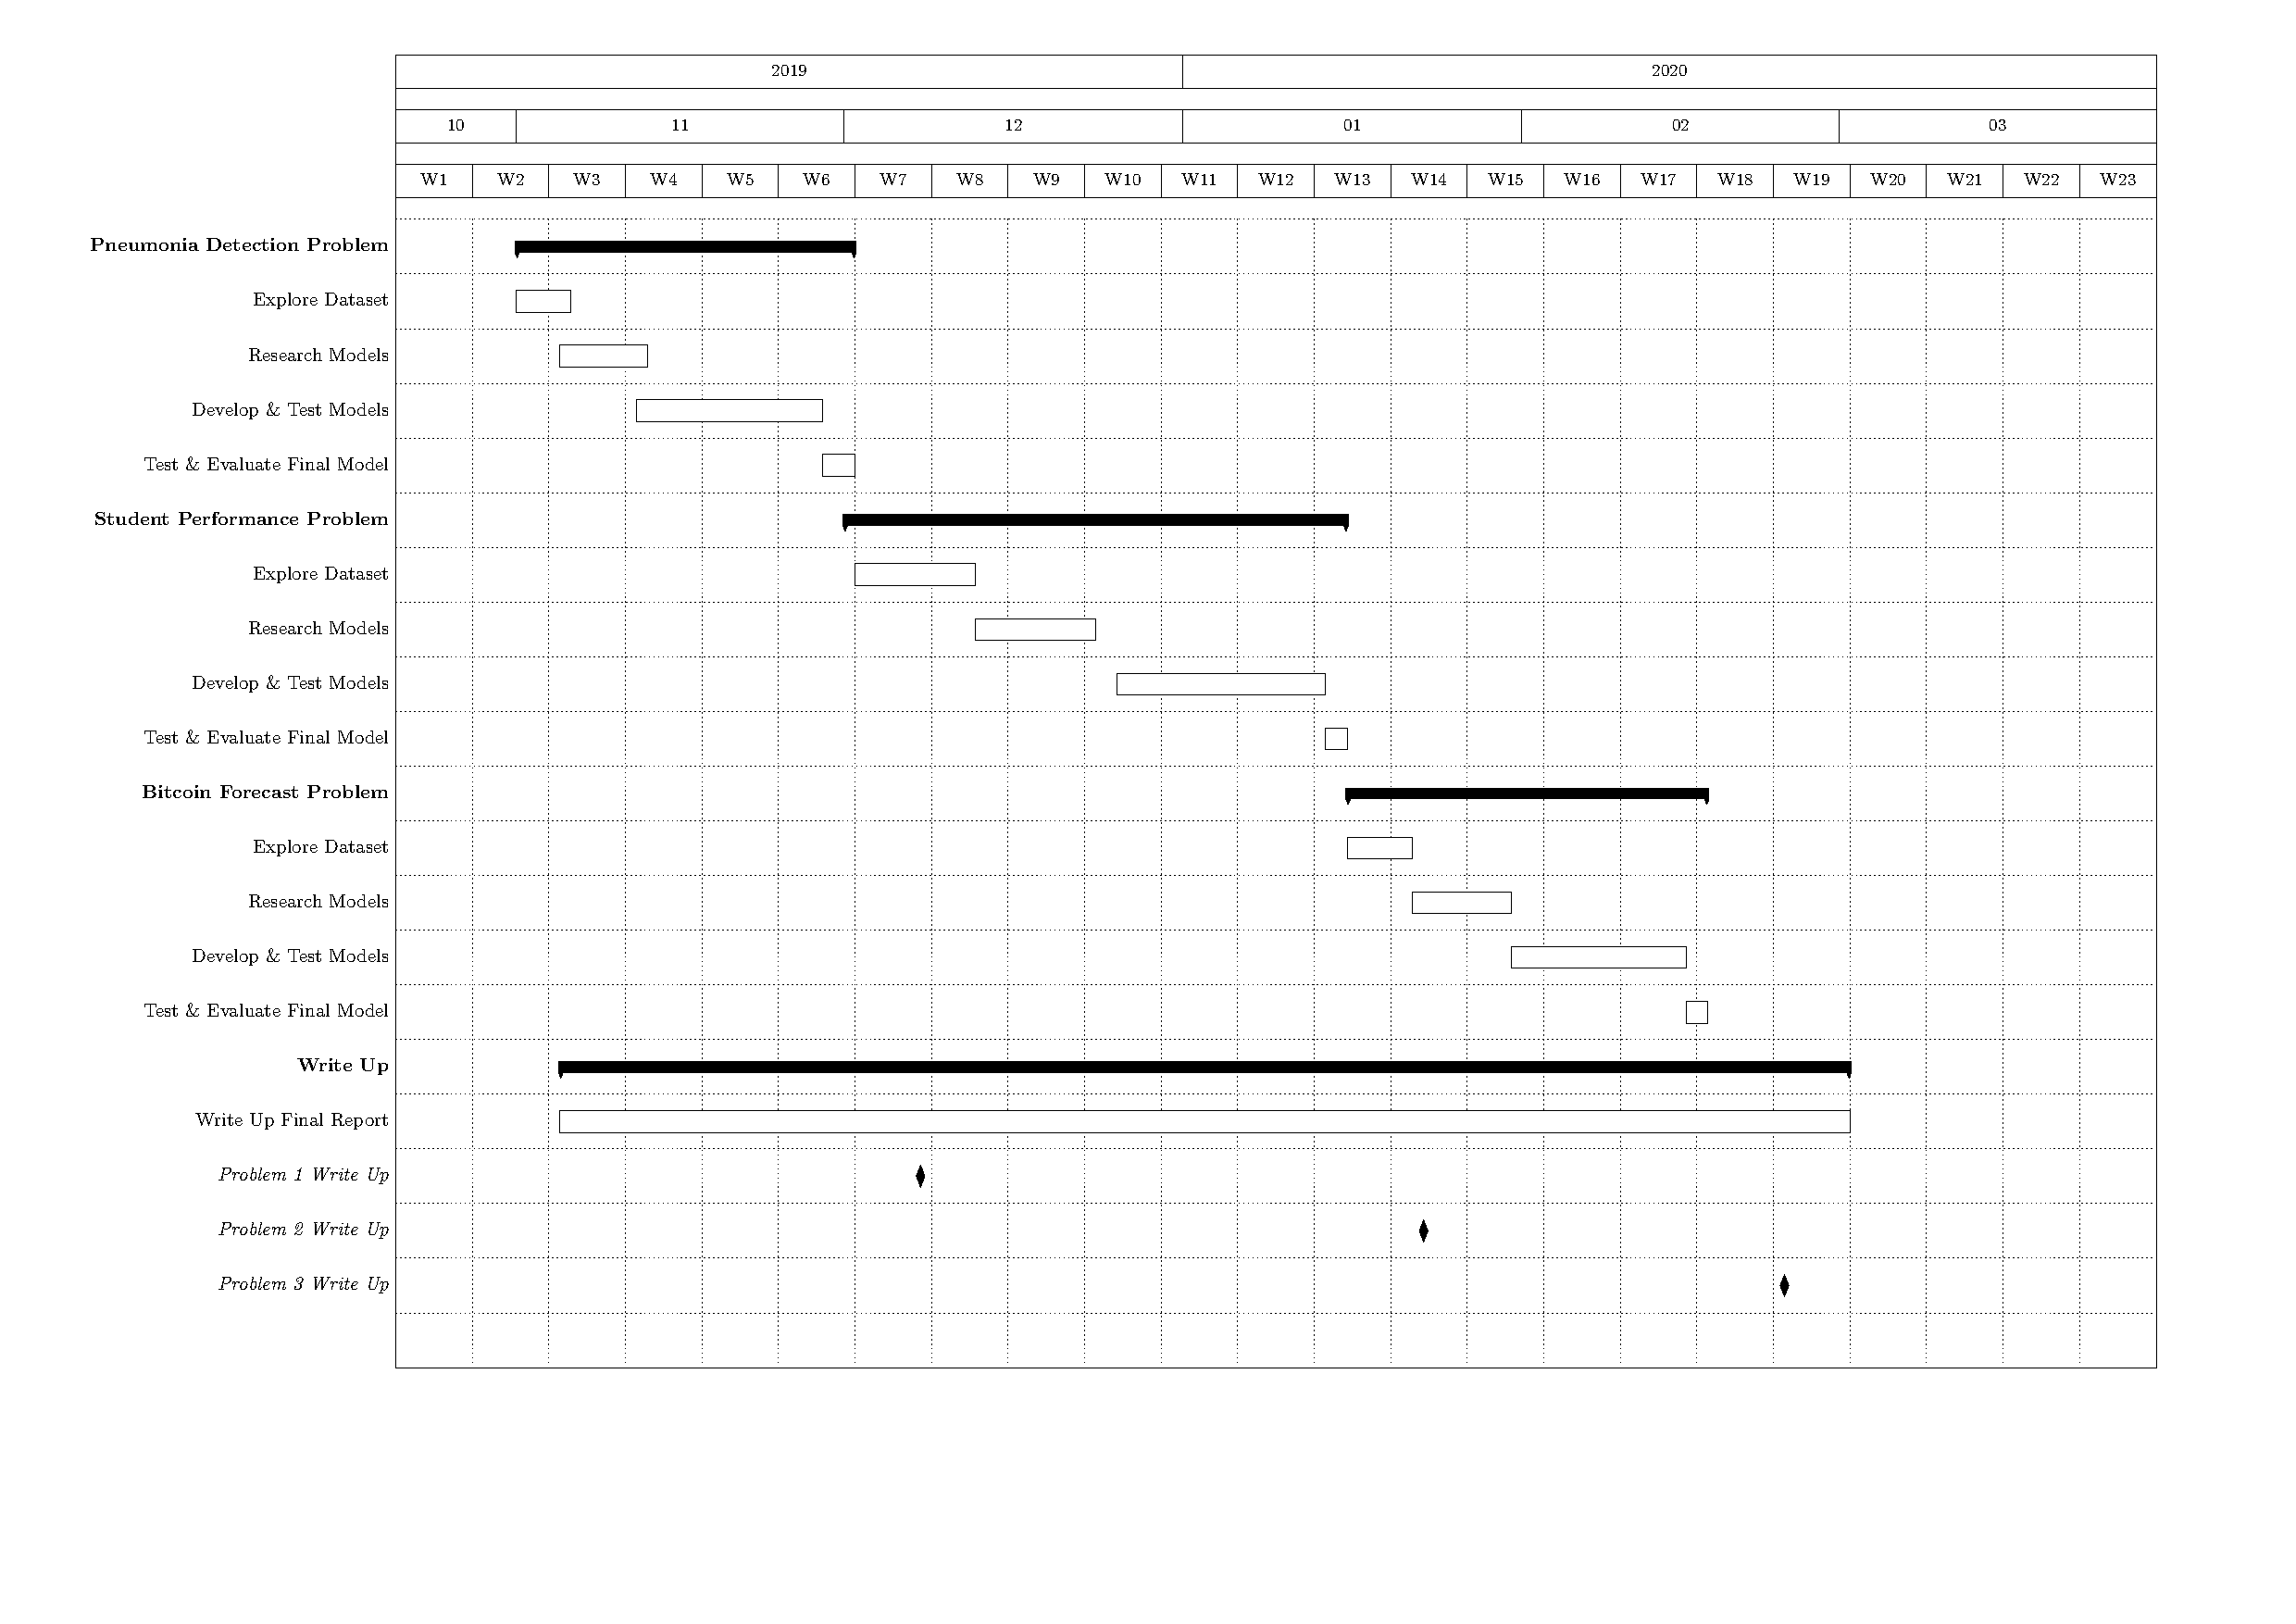
\includepdf[landscape=true]{gantt-chart.pdf}

\chapter{Requirements}
	All software required for this project is free and open-source. There are no real hardware requirements, though an Amazon web-services EC2 instance will be used to speed up training times.
\begin{itemize}
\item Python (version 3.6)
\item Scikit-learn (version 0.21.3)
\item Keras (version 2.2.4 (TensorFlow version 1.13.1 backend))
\item AWS EC2 instance (Hardware instance: p2.xlarge, running: Deep Learning AMI (Ubuntu) Version 24.1)
\end{itemize}

\printbibliography


\end{document}
